\newpage
\section{Metodologia Experimental}

    \subsection{Materiais}
        O material utilizado para realização do experimento foi:

        \begin{itemize}
            \item U-2970A Gerador de dados;
            \item U-2970B Formatador de dados;
            \item U-2970C Modulador balanceado duplo;
            \item U-2970D Deslocamento de fase da portadora;
            \item U-2970E Oscilador Controlado por Tensão;
            \item U-2970F Regenerador de clock de dados;
            \item U-2970G Recuperador de dados;
            \item U-2970H Receptor de dados;
            \item U-2970K Módulo de áudio;
            \item U-2970L Circuito de sintonia;
            \item U-2970M Fonte de alimentação;
            \item U-2970N Conjunto de cabos de alimentação;
            \item Osciloscópio de 2 canais.
        \end{itemize}

        Para execução do experimento, faz-se necessário executar os passos descritos a seguir.

    
    \subsection{Modulação PSK}
        \begin{enumerate}
	        \item Conectar os equipamentos conforme mostrado na Figura \ref{fig:montagem}(a).
	        
	        \item Notar que a forma de onda do dado bi-fase do módulo de formato de dados U-2970B sempre tem a mesma componente DC médio ao longo de um tempo de bit. Pode-se verificar isso medindo-se sua componente DC com um voltímetro. Por isso, a alimentação do capacitor do modulador pode rejeitar o nível DC e produzir iguais entradas positivas e negativas para o modulador apropriado. Cheque isto com o osciloscópio na entrada b.
	        
	        \item Usar o osciloscópio para verificar que o U-2980D produz deslocamento de fase na forma de onda da portadora em mútua quadratura nas ligações 10 e 12. O controle de ganho associado pode ser girado totalmente no sentido horário e o controle de fase deve ser ajustado inicialmente para dar aproximadamente a mesma tensão de saída.
	        
	        \item Estas duas tensões são alimentadas respectivamente por dois moduladores. O modulador inferior tem uma constante de nível DC como sua segunda saída, de modo que, sua saída corresponde ao fasor C na figura 1. O controle do nível DC controla a magnitude desta saída. Isto deve ser configurado para um valor positivo girando o controle no sentido horário. A ligação 10 fornece a portadora em quadratura que é invertida em fase como o sinal modulado (ligação 9) troca o sinal no terminal b.
	        
	        \item A corrente de saída dos dois moduladores são combinadas na carga comum produzindo o sinal modulado em fase.
	        
	        \item O sinal modulado em fase pode ser examinado da seguinte forma:
		        
		        \begin{enumerate}
		        	\item aumentar a velocidade da base de tempo para $2 \mu s$ por divisão;
		        	
		        	\item sincronizar (usando a conexão do \textit{trigger} externo por melhor conveniência) para portadora de $1,28MHz$, ligação 6, ao qual o canal CH1 também deve ser conectado;
		        	
		        	\item finalmente exibir a saída, ligação 14, no canal CH2.
		        \end{enumerate}
			    
	        \item Isto mostrará as duas fases sobrepostas na saída. A quantidade de modulação pode ser variada pelo ajuste no controle da fase. Isto deve ser configurado para menor do que $\pm 90º$.
	        
	        \item Deve-se observar o efeito da limitação da largura de banda na forma de onda da saída. Conectar o módulo do circuito sintonizado U-2970L nos terminais alto e baixo nas ligações 14 e 15 e girar para o sinal máximo. Note a tendência da amplitude e fase do sinal ao passar de estados de transição bastante prolongados, cada vez que os valores dos dados mudam.
        \end{enumerate}
            

            
    \subsection{Demodulação PSK}
                        
        \begin{enumerate}
            \item Sem mexer nos equipamentos já instalados (incluindo o osciloscópio) conectar o restante como mostrado na Figura \ref{fig:montagem}(b). As ligações 14 e 15 são os enlaces de comunicação e são, por conseguinte, as mesmas ligações 14 e 15 mostradas na Figura \ref{fig:montagem}(a).
            
            \item Com o sinal na ligação 14, transferir o CH1 (mas não mudar o \textit{sync}/\textit{trigger}) para o módulo VCO, ligação 16. Deve-se observar a portadora recuperada do sinal pelo PLL. Isto irá variar um pouco em fase, mas não muito porque embora o circuito tenta bloquear a mudança de fase do sinal de entrada, esta ação é lenta.
            
            \item Observar que sua fase está em quadratura com a fase média do sinal recebido. As componentes em quadratura desse último (Q na Figura \ref{fig:fasor}) são portanto $0º$ ou $180º$. Uma senóide multiplicada por outro de mesma fase produz uma componente DC na saída:
            
            \begin{equation}
	            2sin^2(\omega t) = 1 - cos(2 \omega t).
            \end{equation}
            
            \item Quando um desses é atrasado de $180º$ esta componente muda de sinal. A saída do modulador nas ligações 20 e 21, portanto, contém componentes que representam os dados bi-fase originais. No capacitor de derivação passa mais as componentes de frequência $2 \omega t$, mantendo a tensão de \textit{ripple} pequena.
            
            \item Checar isto com o osciloscópio, CH1 mostrando os dados bi-fase na ligação 9 e CH2 os dados recuperados na ligação 20. As configurações devem ser restauradas para o seguinte:
	        \begin{enumerate}
	            \item CH1 e CH2: acoplamento DC, $5V/divisão$;
	            	
	            \item base de tempo: $10 \mu s/divisão$, \textit{triggered} externamente pelos extremos $\pm V E$.
	        \end{enumerate}

            \item Verificar que este sistema não é adequado para PSK de $\pm 90º$. Para fazer isto, primeiro configure um padrão de dados simples (tal como um simples conjunto de bits 1) e verificar sua recepção na recepção dos dados. Remover a ligação 1. E então, ajustando o controle de ganho e de fase no deslocamento de fase da portadora U-2970D, aumentar o deslocamento de fase acima de $\pm 90º$. Observe que como o deslocamento de fase passa através deste valor crítico o dado é complementado de modo que ocorre o chaveamento de exatamente $\pm 90º$, a geração de fase pelo modulador inferior varia de forma aleatória.
        \end{enumerate}
        
         \begin{figure}[H]
           	\centering
           	\caption{Montagem do: a) Transmissor PSK; b) Receptor PSK.}
           	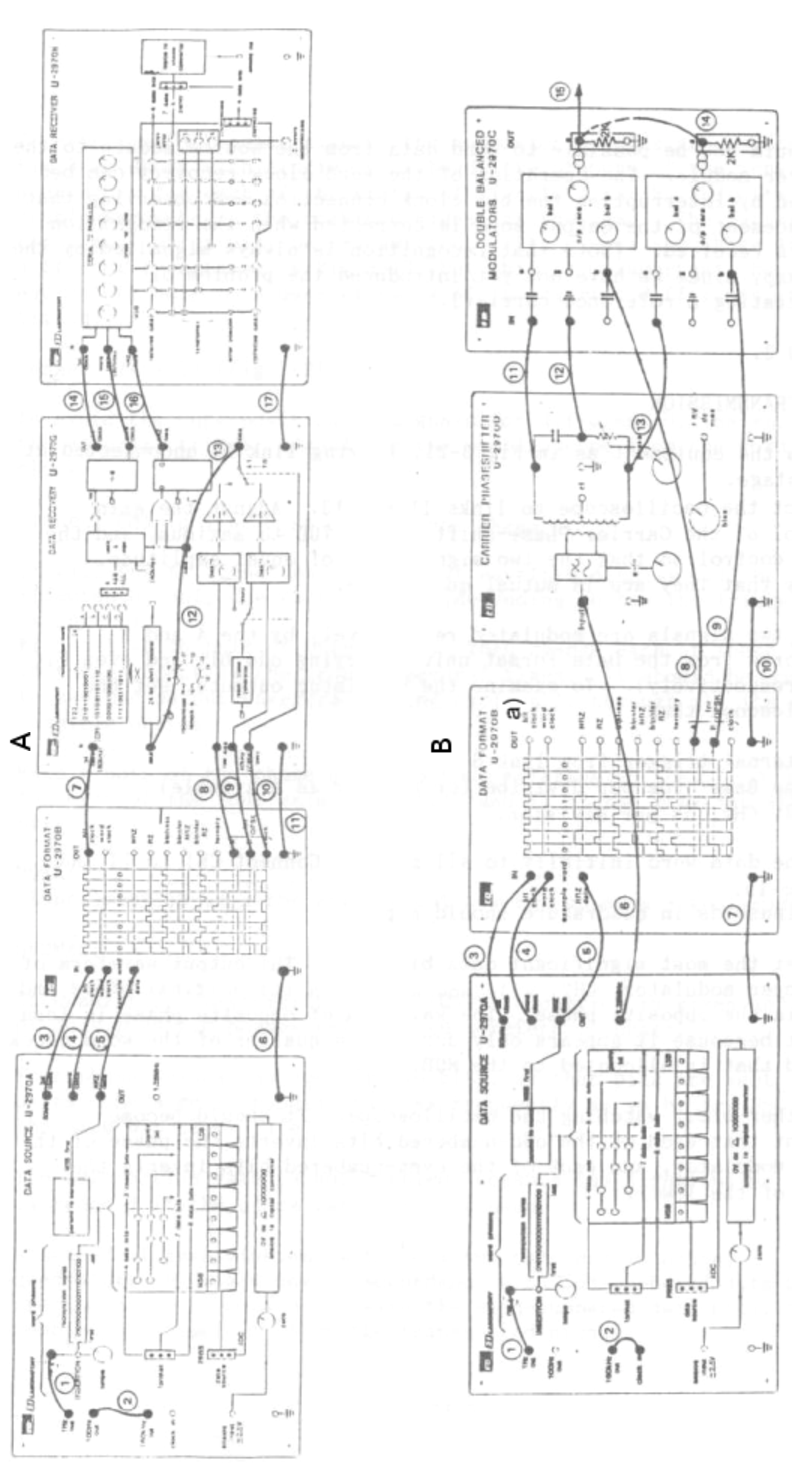
\includegraphics[scale=0.45]{montagem}
           	
           	\small Fonte: Jacob, J. L., Roteiro de laboratório, 2017 [1].
           	\label{fig:montagem}
         \end{figure}